\section{Optimización intertemporal y la aversión al cambio}

El economista y estadístico \textbf{Irving Fisher}\marginnote{\textbf{Irving Fisher 1867-1947:} Economista y estadístico estadounidense reconocido por sus avances en la teoría económica (Ecuación de Fisher, hipótesis de Fisher, teorema de separabilidad de Fisher...).} ayudó a desarrollar uno de los modelos más influyentes en como entendemos que se toman las decisiones de consumo a lo largo del tiempo. El objetivo es entender lo que lleva a individuos a suavizar el consumo a través del tiempo reconociendo también los factores que impulsan el consumo hacía el presente mediante deuda o al futuro mediante ahorros.

La sustancia del modelo es un consumidor racional que maximiza su utilidad sujeto a ciertas restricciones. Las restricciones de cada período tales como ingreso, pueden ser unificadas mediante el ahorro o la deuda que haya tomado el individuo en algun momento del tiempo, por lo que se puede escribir una gran restricción intertemporal que considera el ingreso e intereses que cobra o paga el individuo a lo largo de su vida. 

Los tres factores principales que es importante notar en las siguientes partes de esta sección será que (i) el individuo busca suavizar el consumo dadas ciertas funciones de utilidad, es decir consumir cantidades similares en cada período, (ii) el costo de la deuda y el premio del ahorro llevarán a consumir más en el futuro y (iii) la impaciencia del individuo llevará a consumir más en el presente.

\subsection{Modelo de consumo intertemporal en dos períodos}

Algunos supuestos simplificadores que asumiremos será que el individuo solo vive durante dos períodos, la tasa de interés no cambia a lo largo del tiempo, la tasa de interés del ahorro es igual a la del consumo. Partiremos armando intuitivamente la restricción de cada período para así juntarlas y obtener lo que llamaremos una \textbf{restricción intertemporal}.\marginnote{\textbf{Restricción intertemporal:} Restricción resultante de consumir con un ingresos finitos transferibles entre períodos de tiempo} 

\textsc{Restricción intertemporal}. El consumidor partirá consumiendo en el primer período una cantidad $c_1$, para financiar su consumo recibe de manera exógena un ingreso $y_1$. Lo primero a notar es que el individuo va a estar restringido pues todo consumo debe estar respaldado por algun tipo de riqueza, es decir $y_1 \geq c_1$. El factor intertemporal entra en juega cuando incluímos la deuda y ahorro, este factor ahorro/deuda lo denotaremos por $s$, será $s>0$ cuando se trate de ahorro y será $s<0$ cuando sea deuda. Por lo que la restricción en el primer período no solo considera que el consumo debe estar respaldado por el ingreso, sino que considera que el ingreso puede destinarse a consumo y ahorro, o bien el ingreso se puede complementar con deuda para consumir más en el presente.

Con esto ya podemos definir la restricción en el primer período como la ecuación \ref{eq: rest 1}.
\begin{equation}
    y_1 = c_1+s \label{eq: rest 1}
\end{equation}

En el segundo período la restricción seguirá la misma lógica, lo que hay que considerar adicionalmente es que hay una tasa de interés ($r$) de por medio para cuando uno ahorra o se endeuda. Por lo que los ingresos $y$ en un período, se convertirán en $y(1+r)$ en el siguiente período.

Por lo tanto el ingreso en el segundo período se destina a consumo o a pagar las deudas pendientes, en caso de que el individuo haya ahorrado en el período anterior se podrá consumir más, no solo por la transferencia de dinero del pasado al presente sino que también el premio al ahorro que es la tasa de interés. La restricción del segundo período puede ser descrita como la ecuación \ref{eq: rest 2}.
\begin{equation}
    y_2 = c_2 - s(1+r) \label{eq: rest 2}
\end{equation}

Teniendo las restricciones para los dos períodos podemos describir una restricción intertemporal combinandolas mediante $s$. Para esto reemplazamos $s$ de \ref{eq: rest 1} en \ref{eq: rest 2}.
\begin{equation*}
    y_2 = c_2 - (1+r)(y_1-c_1) 
\end{equation*}

Reordenando podemos encontrar dos expresiones útiles que representan la misma restricción, las dos significan que todo el consumo tiene que ser financiado por ingreso. La expresión \ref{eq: valor futuro} está ordenada de forma que los ingresos presentes sean traídos a \textbf{valor futuro},\marginnote{\textbf{Valor futuro:} El valor que tendrá cierta monto en un período futuro dadas las oportunidades de ahorro/inversión.}[-4cm] mientras que \ref{eq: valor presente} está expresado de forma en que los ingresos futuros sean traídos a \textbf{valor presente}.\marginnote{\textbf{Valor presente:} El valor que tiene cierto monto en el futuro traído a lo que valdría hoy dadas las oportunidades de ahorro/inversión.} Ambas vienen a signficar lo mismo, el consumo debe estar respaldado por algún tipo de riqueza, ya sea ingresos o ahorros.
\begin{align}
    y_1(1+r) + y_2 &= c_1(1+r) + c_2 \label{eq: valor futuro} \\
    \quad & \quad \notag\\
    y_1 + \frac{y_2}{1+r} &= c_1 + \frac{y_2}{1+r} \label{eq: valor presente}
\end{align}
Si quisieramos graficar deberíamos tomar en el eje horizontal el consumo presente y en el eje vertical el consumo futuro, de esta manera la restricción intertemporal puede ser graficada tal como una restricción presupuestaria (Véase la figura \ref{fig: restricción intertemporal}). De estos puntos factibles el consumidor decidirá el punto de la recta que maximiza su utilidad.
\begin{figure}
    \centering
    \caption{Restricción intertemporal}
    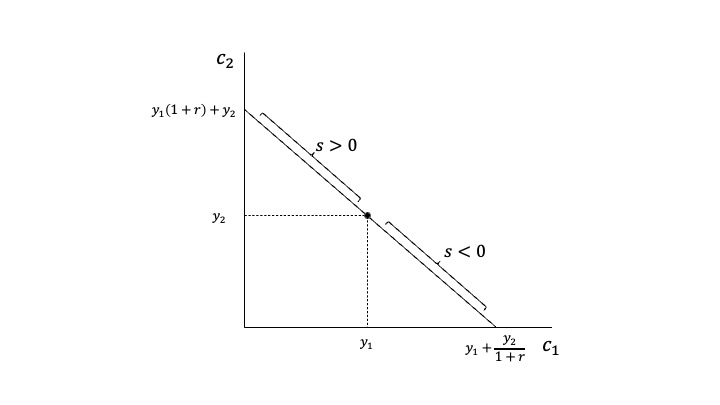
\includegraphics[width=\textwidth]{Figuras/CI Restriccion intertemporal.jpeg}
    \label{fig: restricción intertemporal}
\end{figure}
El punto en que el consumidor elija para maximizar su utilidad es suficiente para saber si en su vida ahorro o se endeudó. Es directo ver que si $c_1>y_1$ implica que $s<0$, es decir se está contrayendo deuda para financiar el consumo presente. Para financiar esa deuda el consumidor estará obligado en el futuro a que $c_2<y_2$ pues cierta parte va a ser usada para pagar la deuda. Tanto este caso como el caso en que el individuo ahorra se pueden ver en la figura \ref{fig: restricción intertemporal}. 

% Falta por mencionar interceptos de los gráficos

Un caso que se verá más adelante son las restricciones de liquidez, es decir cuando la tasa a la que uno se endeuda es más alta a la cual uno ahorra.\footnote{Un caso extremo en que la tasa a la que uno se endeuda tiene a infinito llevará inevitablemente a este consumidor racional a comportarse como un consumidor keynesiano.} 

Ya vimos un punto a considerar mencionados al inicio, el costo de la deuda y el premio del ahorro llevan consumir más en el futuro. Un ingreso $y$ ahora que se ahorra será $y(1+r)$ en el siguiente período, por lo cual podríamos consumir más en el futuro. Entonces ¿Por qué el consumidor no ahorra todo su ingreso al inicio para maiximizar el ingreso y por tanto el consumo que le da felicidad? Para responder esta pregunta es necesario tomar en consideración los puntos que nos faltan que se relacionan con las preferencias del individuo por suavizar el consumo y las de impaciencia. 

\textsc{El Consumidor}. Podemos expresar la función de utilidad entre los dos períodos en la ecuación \ref{eq: ut intertemporal}.
\begin{equation}
    U(c_1,c_2) = u(c_1) + \frac{1}{1+\rho} u(c_2) \label{eq: ut intertemporal}
\end{equation}
Vemos que se compone de dos funciones de utilidad para cada período y un factor de descuento. Primero analicemos las funciones de utilidad para entender porque el consumidor tiende a suavizar el consumo. Las funciones de utilidad para cada período $i$ serán tal que $u'(c_i)>0$ y $u''(c_2)<0$, es decir, cada unidad de consumo aumentará la utilidad en ese período pero a rendimientos decrecientes. La concavidad de la función de utilidad se puede interpretar como que el individuo es saciable, llegará un punto en que en vez de consumir esa unidad extra hoy conviene consumirla mañana, pues en el total será una mayor utilidad.

A pesar de que la utilidad en el presente y futuro sigan una misma función $c(\cdot)$ el consumidor preferirá el consumo presente por sobre el consumo en futuro. Para incluir esta impaciencia se añade una \textbf{tasa de impaciencia} que descontará la utilidad del consumo en futuro. Dado que $\rho>0$ tendremos que se pondera al utilidad en el futuro por un número menor a 1. Por conveniencia podemos hacer un cambio de variable y definir $\beta = \frac{1}{1+\rho}$. 

Dado que tenemos la utilidad y restricción intertemporal podemos plantear el problema de maximización que enfrenta el individuo.
\begin{align*}
        \max_{c_1,c_2} & \quad \Bigl\{ u(c_1) + \beta u(c_2) \Bigr\} \\ s.a.& \quad  y_1 + \frac{y_2}{1+r} = c_1 + \frac{c_2}{1+r}
\end{align*}
Para resolver este problema definimos el lagrangeano y derivamos las condiciones de primer orden. 
\begin{align}
        \mathcal{L}:& u(c_1) + \beta u(c_2) + \lambda \left( y_1 + \frac{y_2}{1+r} - c_1 - \frac{c_2}{1+r} \right) \notag \\
        \text{CPO:} \quad & \frac{\partial \mathcal{L}}{\partial c_1} = u'(c_1) - \lambda = 0 \notag \\
        &\frac{\partial \mathcal{L}}{\partial c_2} = \beta u'(c_2) - \frac{\lambda}{1+r} = 0 \notag \\
        & \lambda = \lambda \longrightarrow u'(c_1) = \left( \frac{1}{1+\rho} \right) u'(c_2)(1+r) \notag \\
        &  \frac{u'(c_1)}{u'(c_2)} = \frac{1+r}{1+\rho} \label{eq: perfil del consumidor}
    \end{align}
El resultado de la optimización será la ecuación \ref{eq: perfil del consumidor} la cual describe el cómo se ajusta la relación consumo presente y consumo futuro frente a las tasas de interés e impaciencia. Esta ecuación se le conoce como la \textbf{ecuación de Euler del consumo}, se le refiere también como el perfil del consumidor. Por ejemplo, un aumento de la tasa de interés tiene un efecto positivo sobre el consumo futuro en relación con el consumo presente dado que se premía más el ahorro. Que el consumo presente disminuya implica que la utilidad marginal del consumo presente aumente dado que la función de utilidad tiene rendimientos decrecientes. Por el contrario un aumento en la tasa de impaciencia disminuye el consumo futuro de la bajo el mismo mecanismo.

Podemo notar del perfil del consumidor que las tasas de interés e impaciencia son fuerzas que mueven el consumo en sentidos contrarios: La tasa de interés impulsa el ahorro y por tanto el consumo futuro mientras que la tasa de impaciencia incentiva el consumo presente y por tanto la deuda. Podemos conceptualizar los cambios entre consumo presente y consumo futuro como \textbf{efectos sustitución} y \textbf{efecto ingreso} tomando la tasa de interés como el precio relativo del consumo entre períodos. 

El precio relativo de consumo presente en relación al consumo futuro es la tasa de interés puesto que el dinero que no se gaste en el presente será $(1+r)$ más valioso en el futuro. Por tanto un aumento en la tasa de interés se toma como un aumento del precio relativo del consumo presente frente al consumo futuro incentivando el consumo de este último: consumir en el presente es más caro pues está considerando mayor costo de oportunidad del dinero. Por el otro lado habrá un efecto ingreso, personas que tienen ingreso ahorrado ante un aumento de la tasa de interés verán aumentada su riqueza y por tanto tenderán a consumir más en ambos períodos. Por el contrario personas que tienen deudas serán más pobres y por tanto reducirán su consumo en ambos períodos. 
% faltan marginnotes para los conceptos en negrita
La dirección y el tamaño del ajuste ante cambios en el precio relativo del consumo entre períodos se pueden medir, estamos describiendo una elasticidad. Para esto tomamos el logaritmo natural y derivamos parcialmente por el precio relativo.
\begin{align*}
    \ln \left( \frac{u'(c_1)}{u'(c_2)} \right) = \ln (1+r) &- \ln(1+\rho)\\
    \frac{\partial \ln (u'(c_1)/u'(c_2))}{\partial \ln (1+r)}  &= 1
\end{align*}
Vemos que un aumento de un $1\%$ en el precio relativo del consumo entre períodos lleva a un ajuste de $1\%$ en los consumos entre los períodos. Ahora veremos un caso en donde esto no ncesariamente es así, hasta ahora no hemos considerado que las personas son aversas al riesgo. Este factor es ampliamente incluido en diversos modelos macro.

\subsection{Funciones de utilidad con aversión al riesgo}

Un caso especial y muy utilizado para describir el consumo de agentes en la economía es el uso de funciones de utilidad que incluyan aversión al riesgo. Las funciones de aversión relativa al riesgo constante (CRRA) incluyen el factor aversión al riesgo como una variable $\sigma$ que tendrá un efecto sobre la magnitud de los ajustes ante cambios en las variables exógenas (Como la tasa de interés por ejemplo). 

Un función de utilidad CRRA se puede describir como la expresión \ref{eq: CRRA}.
\begin{equation}
    u(c)= \left\{ \begin{array}{lcc} \frac{c^{1-\sigma}-1}{1-\sigma} & \text{si} & \sigma >0,\sigma \neq 1 \\ \\ \ln{(c)} & \text{si} & \sigma = 1 \end{array} \right. \label{eq: CRRA}
\end{equation}

De la cual si resolvemos llegaremos a una ecuación de Euler del consumo de la ecuación \ref{eq: perfil con aversión al riesgo}). De aquí podemos definir la \textbf{elasticidad intertemporal de sustitución} como el cambio porcentual en la relación marginal de consumo 1 y 2 para un cambio del $1\%$ en el precio relativo del consumo en 1 (tasa de interés). 
\begin{equation}
    \left( \frac{u'(c_1)}{u'(c_2)} \right) ^\sigma=  \frac{1+r}{1+\rho}  \label{eq: perfil con aversión al riesgo}
\end{equation}

La elasticidad intertemporal de sustitución describe la magnitud en que el consumo presente y futuro se ajustan ante un cambio en las condiciones (tasa de interés e impaciencia). 
\begin{equation}
    \text{EIS} = - \frac{\partial \ln (u'(c_1)/u'(c_2))}{\partial \ln (1+r)} = \frac{1}{\sigma}
\end{equation}

Mientras mayor sea la aversión al riesgo ($\sigma$) el consumidor responderá en menor medida a cambios en estas variables. Es decir, un aumento de $1\%$ en el precio relativo del consumo presente en relación al consumo futuro tendrá un efecto $1/\sigma$ en la relación de consumo futuro y consumo presente.

Mientras mayor sea la $\sigma$ mayor será la aversión al riesgo, representado por una curva más cóncava. Cuando grafiquemos una función $u(c)$ que sea cóncava está tendrá implícita cierta aversión al riesgo.

\subsection{Restricciones de liquidez}

Hasta ahora se ha asumido que la tasa a la que un individuo ahorra ($r$) y se endeuda ($r^*$) es la misma. Un acercamiento más realista es que la tasa que paga un deudor es mayor a la tasa que consigue alguien por ahorrar. 
% Incluir razones por las que pasa esto

Cuando hablamos de \textbf{restricciones de liquidez} específicamente nos referimos a restricciones al endeudamiento puesto que esta restricción se da solo al momento de endeudarse, las personas que en el neto ahorran no se verán afectadas. Este margen puede deberse a que la tasa de endeudamiento considera un premio por riesgo cuando hay probabilidad de impago. Mercados financieros menos robustos, los cuales suelen estar presentes en países menos desarrollados suelen estar sujetos a mayores restricciones de liquidez, lo cual deriva en muchas implicancias macro y microeconómicas.\footnote{Efectos sobre inversión y aplificación del ciclo económico, racionamiento del crédito, ineficiencias que llevan a perpetuar la desigualdad, etc\ldots}

\begin{figure}[t]
    \centering
    \caption{Restricciones de liquidez y perdida de bienestar ahorradores y deudores}
    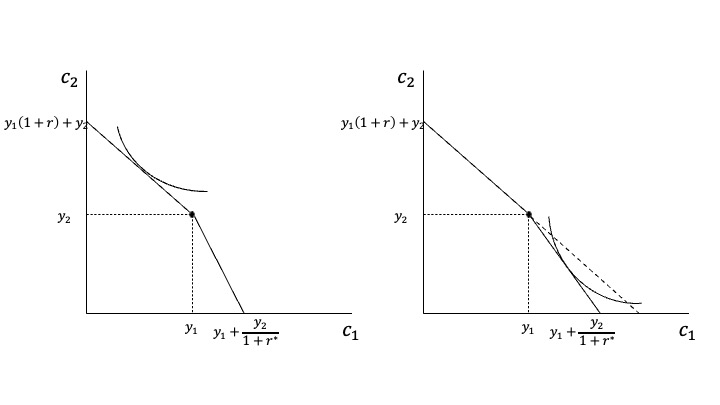
\includegraphics[width=\textwidth]{Figuras/CI Restricciones de liquidez.jpeg}
    \label{fig: Restricciones liquidez bienestar}
\end{figure}

Podemos ver los efectos en el bienestar de un consumidor bajo restricciones de liquidez en dos casos. El caso a la izquierda (Figura \ref{fig: Restricciones liquidez bienestar}) es el consumidor que en el neto ahorra, para este individuo la restricción no está activa puesto que las restricciones de liquidez solo afectan a la tasa de endeudamiento. En el caso de la derecha el individuo en el neto se endeuda y para él la restricción está activa, el punto que maximizaba el bienestar ya no es factible y por tanto hay una perdida en cuanto a utilidad, la curva de indiferencia es de menor nivel. 

Es fácil ver que las restricciones tienen efectos negativos (o nulos) en el bienestar de las personas pues reduce la cantidad de opciones factibles en las que maximizar utilidad. 